\chapter{外文资料的调研阅读报告或书面翻译}

\title{在结构化数据上用随机梯度下降算法学习过参数化神经网络\cite{li2018learning}}

{\heiti 摘要:} 神经网络有许多成功的应用,而理论上的理解却少得多。为了弥补这一缺陷,我们研究了从随机初始化中通过随机梯度下降(SGD)学习用于多类分类的双层超参数ReLU神经网络的问题。在过参数化的情况下,当数据来自分离良好的分布时,我们证明了SGD学习的网络具有较小泛化误差,尽管该网络具有足够的能力来适应任意标签。此外,该分析对学习神经网络的几个方面提供了有趣的见解,并可通过对合成数据和MNIST数据集的实验加以验证。

\section{背景介绍}
神经网络在许多应用中取得了巨大的成功,但尽管最近理论研究有所增加,但仍有许多问题有待解释。例如,根据经验观察,在过参数化设置(即,需要学习的参数数量大于训练数据点数量的大型网络)中使用随机梯度下降(SGD)进行学习不会导致过度拟合[24,31]。一些最近的研究使用低复杂度的学习算法来解释泛化,但通常不能解释SGD或其变体如何支持低复杂度的算法(即,归纳偏差或隐式正则化)[3, 23]。我们还观察到,过参数化和适当的随机初始化有助于优化[28、12、26、18],但也不清楚为什么特定的初始化可以改善学习过程。此外,大部分试图解释这些现象的现有作品依赖于关于数据分布的不切实际的假设,例如高斯性和/或线性可分性〔32, 25, 10,17, 7〕。
\par
因此,本文提出在更真实的数据结构上,研究利用SGD进行分类的两层超参数神经网络的学习问题。特别是,每个类中的数据是几个元素的混合,不同类的元素在距离上有很好的分隔(但是每个类中的元素可以彼此接近)。这是由实际数据驱动的。例如,在数据集MNIST[15]上,每个类对应于一个数字,并且可以具有对应于数字的不同写入样式的多个元素,其中的图像是其中一个元素的小扰动。另一方面,属于同一分量的图像比另一个数字的图像更接近彼此。在此设置中进行分析可以帮助理解实际数据的结构如何影响优化和泛化。
\par
在这种情况下,我们证明了当网络充分过参数化时,可证明SGD可以学习到接近随机初始化且具有小的泛化误差的网络。结果表明,在过参数化的情况下,当数据结构良好时,虽然原则上网络可以过拟合,但随机初始化的SGD引入了很强的归纳偏差,具有很好的泛化能力。
\par
我们的结果还表明,过参数化要求和学习时间取决于数据结构固有的参数,而不是数据的环境维度。更重要的是,通过分析得到的结果也为神经网络学习的各个方面提供了一些有趣的理论见解。它揭示了学习的成功关键依赖于过参数化和随机初始化。这两者结合在一起,导致SGD和另一个具有良性优化环境的学习过程之间的初始化紧密耦合。这种耦合,加上数据的结构,使得SGD能够找到一个具有低泛化误差的解,同时仍然保持在上述初始化的领域内。我们的工作进一步解释了过参数化和随机初始化如何帮助优化,以及结构化数据上的SGD动力学上如何产生归纳偏差和良好的泛化。我们将在稍后的章节中讨论一些其他的技术内含,如在初始化时存在一个好的解,以及学习的权重的低秩性。对综合数据和基准数据集MNIST的补充实证研究为分析和见解提供了积极支持。

\section{相关工作}
\textbf{神经网络的泛化}。实验显示了神经网络泛化的一些有趣现象:实际的神经网络具有拟合随机标签的训练数据的能力,但在训练实际数据时仍具有良好的泛化能力[24,31,2]。由于这些网络的参数比统计上所需的参数多,因此它们是过参数化,而单纯地应用传统理论无法解释其良好的泛化性。多方面的工作提出了一些低复杂度的学习网络和衍生的泛化界限,以更好地解释。[3,23,21]证明了基于谱归一化裕度的泛化界,[9,23]从PAC-Bayes方法导出了界,以及[1,33,4]用压缩方法导出了界。一般来说,他们没有解决为什么会出现低复杂度。本文朝着这个方向迈出了一步,尽管是在两层网络和简化的数据模型上。
\par
\textbf{超参数化和隐式正则化}。过参数化网络的训练目标在原理上具有许多(近似)全局最优解,并且一些推广优于其他14, 8, 2种,而经验观察意味着实践中的优化过程更倾向于那些具有更好泛化性的网络。因此,一个有趣的问题是,这种隐式正则化或归纳偏差是如何从数据的优化和结构中产生的。最近的研究是针对不同任务的SGD,如logistic回归[27]和矩阵分解[11,19,16]。与我们的工作更相关的是[7],它研究了在线性可分数据上学习两层超参数网络的问题,并证明了SGD收敛到全局最优,具有很好的推广性。我们的工作研究了具有良好聚类(并且可能不是线性可分)结构的数据的问题,我们认为这种结构更接近实际情况,因此可以推进这一研究路线。
\par
学习神经网络的理论分析。还存在大量的工作,分析学习神经网络[13, 26, 30,10, 25, 29,6, 32, 17,5]的优化景观。一般来说,他们需要对数据假设不现实的假设,如高斯性,和/或对网络有很强的假设,如仅使用线性激活。他们也没有研究隐式正则化的优化算法。

\section{问题建模}
本文中,我们考虑一个两层的激活函数为ReLU的k-分类神经网络$f = (f_1,f_2,\cdots,f_k)$,满足对$\forall i \in [k]$,有
\[
f_i(x) = \sum_{r = 1}^m a_{i,r} ReLU(\langle w_r, x\rangle)
\]
其中$\{w_r\in \mathbb{R}^d\}$是隐藏层中的$m$个神经元的权重,$\{a_{i,r}\in \mathbb{R}\}$是最后一层的权重,$ReLU(z) = \max\{0,z\}$。
\par
\textbf{对数据的假设:}数据按照以下方式从分布$\mathcal{D}$中产生,一共有$k\times l$个$\mathbb{R}^d$上的未知分布$\{\mathcal{D}_{i,j}\}_{i\in [k] ,j \in [l]}$,和概率$p_{i,j}\geq 0$满足$\sum_{i,j}p_{i,j} = 1$。每个数据都是独立同分布地生成:(1) 取样$z\in [k]\times [l]$满足$Pr[z = (i,j)] = p_{i,j}$;(2) 设置标签$y = z[0]$,从分布$\mathcal{D}_z$中取样$x$。假设我们取了$n$个样$\{(x_i,y_i)\}_{i=1}^n$。
\par
让我们定义密度$\rho$在$\mathbb{R}^d$的分布$\mathcal{D}$的支撑集为$supp(D) = \{x:p(x)>0\}$,两个集$S_1,S_2\subset \mathbb{R}^d$之间的距离为$dist(S_1,S_2)= \min_{x\in S_1,y\in S_2}\{\|x–-y\|_2\}$,集$S_1\subset \mathbb{R}^d$的直径为$diam(S_1) = \max_{x,y\in S_1}\{\|x-y\|_2\}$。然后我们准备对数据进行假设。
\begin{itemize}
  \item[\textbf{A1}] (可分离性)存在$\delta >0$满足对任意的$i_1\neq i_2\in[k]$和任意的$j_1,j_2\in[l]$,$dist(supp(\mathcal{D}_{i_1,j_1}), supp(\mathcal{D}_{i_2,j_2}))\geq \delta$。除此之外,对任意的$i\in [k],j\in [l]$,$diam(supp(\mathcal{D}_{i,j}))\leq \lambda \delta$,其中$\lambda \leq 1/(8l)$。
  \item[\textbf{A2}] (正则性)对任意的$x$有$\|x\|_2 = 1$。
\end{itemize}
\par
有一些重要的记述。我们考虑的不是一个类只有一个分布,而是在每个类中有一个任意的$(l\geq 1)$分布,我们认为这更吻合实际数据。例如,在MNIST中,一个类可以是数字1,而l可以是不同的书写风格1(1或|或/)。
\par
假设(A2)是为了简单起见,而(A1)是我们的关键假设。当每个类中有$l \geq 1$分布时,我们的假设数据是不可线性分离的,例如$\mathbb{R}^d$中有两个类的异或型数据,一个类由两个直径为1/10的球组成,球的中心为(0,0)和(2,2),另一个类由两个直径相同的球组成,球的中心为(0,2)和(2,0)。有关说明请参见附录C中的图3。此外,我们这里唯一的假设是$\lambda = O(1/l)$。当$l=1$时,$\lambda = O(1)$,这是分布可被有效学习对$\lambda$的阶的最小要求。我们的工作允许更大的$l$,因此每个类中的数据可能更复杂。在这种情况下,我们对数据的可分离性的要求也更高。当我们增加$l$来细化每个类内的分布时,每个分布的直径应该也变小。只要每个分布的直径递减率大于分布的总数,那么我们的假设就成立。
\par
\textbf{关于学习过程的假设。}我们将只学习权重$w_r$来简化分析。由于ReLU激活函数是正单调的,所以过参数化的影响仍然可以研究,并且在以前的工作中已经采用了类似的方法[7]。所以网络也可写为$y = f(x,w) = (f_1(x,w),\cdots,f_k(x,w))$,其中$w = (w_1,\cdots, w_r)$。
\par
我们假设学习过程的初始化为随机的:
\begin{itemize}
  \item[(A3)](随机初始化)$w_r^{(0)}\sim \mathcal{N}(0,\sigma^2I), a_{i,r} \sim \mathcal{N}(0,1)$,其中$\sigma = \frac{1}{\sqrt{m}}$.
\end{itemize}
\par
学习过程最小化softmax函数的交叉熵,定义为:
\[
L(w) = -\frac{1}{N}\sum_{s = 1}^N \log o_{y_s}(x_s,w)
\]
其中$o_y(x,w) = \frac{e^{f_y(x,w)}}{\sum_{i=1}^k e^{f_i(x,w)}}$
\par
记$L(w,x_s,y_s) = -\log o_{y_s}(x_s,w)$记为单点$(x_s,y_s)$的交叉熵。
\par
我们把一个批量大小为$B$,迭代次数$T=N/B$,学习率$\eta$的小批量SGD看作如下过程:将训练样本随机分为$T$个批量,每个批量为$B$,让$T$个批量中的样本指标为$B_t$,每次迭代时,更新次数为
\[
w_r^{(t+1)} = w_r^{(t)} -\eta\frac{1}{B}\sum_{s\in \mathcal{B}_t} \frac{\partial L(w^{(t)},x_s,y_s)}{\partial w_r^{(t)}}, \forall r \in [m]
\]
其中
\[
\frac{\partial L(w,x_s,y_s)}{\partial w_r} = \bigg(\sum_{i\neq y_s} a_{i,r}o_i(x_s,w)-\sum_{i\neq y_s} a_{y_s,r}o_i(x_s,w)\bigg)
\]


\section{主要结果}
为了简化记号,对于目标误差$\epsilon$,以大概率的意思是以概率$1-1/poly(1/\delta,k,l,m,1/\epsilon)$为足够大的多项式,$\tilde{O}$忽略了$poly(\log(1/\delta),\log k, \log l, \log m,\log (1/\epsilon))$的因子。
\begin{theorem}
假设满足(A1)(A2)(A3)。那么对于每一个$\epsilon > 0$,$M = poly(k,l,1/\delta,1/\epsilon)$,满足对任意的$m\geq M$,在进行小批量SGD之后,批量大小为$B=poly(k,l,1/\delta,1/\epsilon,\log m)$,学习率$\eta = \frac{1}{m\cdot poly(k,l,1/\delta,1/\epsilon,\log m)}, T = poly(k,l,1/\delta,1/\epsilon,\log m)$次迭代,以高概率:
\[
Pr_{x,y\sim \mathcal{D}}[\forall j \in [k], j\neq y, f_y(x,w^{(T)}) > f_j(x,w^{(T)})] \geq 1-\epsilon 
\]
\end{theorem}
\par
我们的定理意味着如果数据满足我们的假设,并且我们对网络进行了适当的参数化,那么我们只需要在$k,l,1/\delta$的多个样本中使用多项式就可以获得良好的预测误差。这种误差是在真实分布$\mathcal{D}$上直接测量的,而不仅仅是在用于训练该网络的输入数据上。我们的结果也是无维度的:没有依赖于数据的基础维度$\mathcal{D}$,复杂性完全被$k,l,1/\delta$所俘获。此外,不管网络被过度参数化,它只会增加$\log m$的因子的总迭代,因此我们可以通过子指数量过参数化而不显著增加复杂性。
\par
此外,我们可以将每个输入示例视为单个分布,因此$\lambda$始终为零。在这种情况下,如果我们使用批处理大小$B$进行$T$迭代,那么我们将得到$l=N=BT$。然后我们的定理表明,只要$m=poly(N,1/\delta^\prime)$,其中$\delta^\prime$是每个示例之间的最小距离,我们实际上可以拟合输入数据的任意标签。然而,由于总迭代仅依赖于$\log m$,当$m=poly(N,1/\delta^\prime)$,但输入数据是实际结构化的($k,l$和$\delta$都很小)时,即使网络有足够的能力来适应训练示例的任意标签(SGD也可以这样做),SGD实际上也可以实现小的泛化误差。因此,我们证明了SGD对结构化数据具有很强的归纳偏向性:它没有找到一个适合任意标签的坏的全局最优解,而是找到那些具有良好泛化保证的全局最优解。这对[24,31]中的经验观察给出了更为彻底的解释。

\section{直观解释和简化情形的证明概要}
要训练具有ReLU激活的神经网络,需要解决两个问题:
\begin{enumerate}
\item 为什么SGD可以优化训练损失?或者找到一个临界点?由于下卧网络是高度非光滑的,现有定理没有给出任何具有Relu激活的神经网络的SGD的有限收敛速度。
\item 为什么经过训练的网络可以泛化?即使容量足够大,可以容纳输入数据的随机标签?这就是所谓的SGD的感应偏压。
\end{enumerate}
\par
这项工作朝着回答这两个问题迈出了一步。研究表明,当网络参数过高时,网络变得更为“伪光滑”,这使得SGD更容易将训练损失降到最小,而且不会对泛化误差造成影响。我们的证明基于以下重要观察:
\begin{itemize}
  \item 我们越是过度参数化网络,一个神经元和一个数据点的激活模式在固定次数的迭代中改变的可能性就越小。
\end{itemize}
\par
这个观察使我们能够将真实神经网络的梯度与“伪梯度”耦合起来,其中每个数据点和每个神经元的激活模式是固定的。也就是说,当计算“伪梯度”时,对于固定$R,i$,在第$i$个数据点席上是否激活第$R$个隐节点,对于不同的$T$,总是相同的(但对于固定的$T$,对于不同的$R$或$I$,符号可以是不同的)。我们可以证明,除非泛化误差小,否则“伪梯度”总是会出现。做大点。此外,我们还证明了该网络实际上是光滑的,因此SGD可以使损失最小化。
\par
然后我们证明,当隐神经元的数目$m$增加时,在适当降低学习率的情况下,使损失最小化所需的迭代总数基本不变。但是,我们可以将真实梯度与伪梯度耦合的迭代总数增加。因此,有一个多项式大$m$,这样我们可以耦合这两个梯度,直到网络达到一个小的泛化误差。

\subsection{一个简化情形:无方差}
在这里,我们演示了一个简化案例的证明草图,附录a提供了证明。一般情况的证明见附录B。在简化情况下,我们进一步假设:
\begin{itemize}
\item[\textbf{(S)}](无方差)每个$\mathcal{D}_{a,b}$是一个单独的数据点$(x_{a,b},a)$,而且我们正在做与小批量SGD相反的全批量梯度下降。
\end{itemize}

\par
我们重新记损失函数为$L(w) = \sum_{a\in[k],b\in[l]}p_{a,b} L(w,x_{a,b},a)$,且梯度为
\[
\frac{\partial L(w)}{\partial w_r} = \sum_{a\in[k], b\in [l]}p_{a,b}\bigg(\sum_{i\neq a}a_{i,r}o_i(x_{a,b},w) - \sum_{i\neq a} a_{a,r}o_i(x_{a,b},w)\bigg)\mathbb{I}\{\langle w_r, x_{a,b}\rangle \geq 0\}x_{a,b}
\]
\par
我们如下定义伪梯度:
\[
\frac{\tilde{\partial} L(w)}{\partial w_r} = \sum_{a\in[k], b\in [l]}p_{a,b}\bigg(\sum_{i\neq a}a_{i,r}o_i(x_{a,b},w) - \sum_{i\neq a} a_{a,r}o_i(x_{a,b},w)\bigg)\mathbb{I}\{\langle w_r^{(0)}, x_{a,b}\rangle \geq 0\}x_{a,b}
\]
其中我们用$\mathbb{I}\{\langle w_r^{(0)}, x_{a,b}\rangle \geq 0\}$代替真梯度中的$\mathbb{I}\{\langle w_r, x_{a,b}\rangle \geq 0\}$。即,激活状态由初始状态决定。直观上,伪梯度是一个伪网络$g$中的梯度(但是并不完全一样),定义为$g_i(x,w) = \sum_{r = 1}^m a_{i,r}\langle w_r, x\rangle \mathbb{I}\{\langle w_r^{(0)},x\rangle\geq 0\}$.
\par
耦合两个梯度则相当于耦合两个网络。
\par
为了简化,让$v_{a,a,b} = \sum_{i\neq a} o_i(x_{a,b},w) = \frac{\sum_{i\neq a} e^{f_i(x_{a,b},w)}}{\sum_{i=1}^k e^{f_i(x_{a,b},w)}}$,当$s\neq a,v_{s,a,b} = -o_s(x_{a,b},w) = -\frac{f_s(x_{a,b},w)}{\sum_{i=1}^k e^{f_i(x_{a,b},w)}}$。粗略地说,如果$v_{a,a,b}$小时,$f_a(x_{a,b},w)$相较于其他$f_i(x_{a,b},w)$来说较大,所以分类误差较小。
\par
我们证明了以下两个主要引理。第一种说法是,在每次迭代中,其梯度可以与伪梯度耦合的隐藏单元的总数是相当大的。

\begin{lemma}
初始化以大概率,当$\tau>0$,对任意的$t = \tilde{O}(\frac{\tau}{\eta})$,我们有对至少$1-\frac{e\tau kl}{\sigma}$比例的$r\in [m]: \frac{\partial L(w^{(t)})}{\partial w_r} = \frac{\tilde{\partial}L(w^{(t)})}{\partial w_r} $
\end{lemma}
\par
第二条引理说明伪梯度较大除非误差较小。
\begin{lemma}
对$m = \tilde{\Omega}(\frac{k^3 l^2}{\delta})$,对所有的$\{p_{a,b}v_{i,a,b}\}_{i,a\in[k],b\in[l]}\in[-v,v]$,满足$\max \{p_{a,b}v_{i,a,b}\}_{i,a\in[k],b\in[l]} = v$,存在至少$\Omega(\frac{\delta}{kl})$比例的$r\in[m]$满足$\|\frac{\tilde{\partial} L(w)}{\partial w_r}\|_2 = \tilde{\Omega}(\frac{v\delta}{kl})$
\end{lemma}
\par
现在我们展示利用这两个引理证明对一个足够小的学习率$\eta$算法可以收敛。为了简单起见,假设$kl/\delta = O(1),\epsilon = o(1)$。 因此通过引理5.2我们知道除非$v\leq \epsilon$,存在$\Omega(1)$比例的$r$满足$\|\tilde{\partial}L(w)/\partial w_r\|_2 = \Omega(\epsilon)$。除此之外,通过引理5.1我们之道可以选取$\tau = \Theta(\sigma\epsilon)$即$e\tau/\sigma = \Theta(\epsilon)$,这说明存在$\Omega(1)$比例的$r$满足$\|\tilde{\partial}L(w)/\partial w_r\|_2 = \Omega(\epsilon)$。对于足够小的学习率$\eta$,一步的梯度下降会使$L(w)$下降$\Omega(\eta m \epsilon^2)$,所以算法在$t = O(1/\eta m \epsilon^2)$次迭代后会收敛。最后我们只需说明$1/\eta m \epsilon^2\leq O(\tau/\eta) = \Theta(\sigma\epsilon/\eta)$,所以我们始终可以应用引理5.1。因为$\sigma = \tilde{O}(1/\sqrt{m})$,我们知道只要$m\geq poly(1/\epsilon)$。一个小的$v$可以使得泛化误差也很小。

\section{关于分析中的原理的讨论}
我们的分析虽然是为了在结构良好的数据上学习两层网络,但也为在更一般的环境下学习神经网络提供了一些启示。
\par
一般化。最近几行的工作解释了学习网络的低复杂度的泛化网络的泛化现象,从频谱归一化边缘[3, 23, 21]、压缩[1, 33, 4]和PAC Bayes[9, 23]的观点来看。
\par
我们的分析已经部分地解释了如何结构化数据上的SGD(适当的随机初始化)导致从压缩和PCA贝叶斯点视图的低复杂度。我们已经证明,在随机初始化的一个邻域中,w.h.p.梯度与另一个良性学习过程的梯度相似,因此SGD可以在仍然处于邻域中的情况下减小误差并获得一个好的解。接近初始化意味着权重(或者更准确地说,学习的权重和初始化之间的差异)可以很容易地压缩。事实上,在文献[22,1]中,我们已经进行了经验观察,并将其与泛化联系起来。此外,[1]使用helper字符串显式地指出了这种压缩(与我们设置中的初始化相对应)。[1] 同时指出压缩视图可以看作是PAC-Bayes视图的一种更为明确的形式,因此我们的直觉也适用于后者。
\par
在初始化过程中存在一个小的泛化误差的解决方案本身并不明显。直观地说,在结构化数据上,更新是分布在隐藏神经元权重上的结构化信号。然后对于预测,权值中的随机初始化部分具有很强的对消性,而权值中的结构化信号部分共同影响输出。因此,后者可以比前者小得多,而网络仍然可以给出准确的预测。换言之,在离初始化不远的地方可能有一个高概率的解决方案。

\par
对权重的低阶提供了一些见解。更确切地说,当数据被良好地聚集在几个模式周围时,累积的更新(学习权重和初始化之间的差值)应该是近似低秩的,这可以从检查SGD更新看出。然而,当与初始值相比差异很小时,最终权重矩阵的谱由初始值的谱支配,因此将趋向于更接近随机矩阵的谱。同样,这些观察/直觉已经在文献中提出,并且与压缩和泛化(例如,[1])相关。
\par
数据的隐式正则化v.s.结构。已有的工作已经分析了SGD在Logistic回归(27)、矩阵分解(11, 19, 16)和线性可分数据(7)上学习两层网络的隐式正则化。我们的设置和分析技术与现有的工作相比是新颖的。研究结构化数据的一个动机是理解结构化数据在隐式正则化中的作用,即观察到在较少结构化甚至随机数据上学习的解远离初始化。事实上,我们的分析表明,当网络大小是固定的(并且充分过参数化)时,对结构较差的数据(较大的K和‘)的学习需要更多的迭代,因此该解决方案可以更多地偏离初始化,并且具有更高的复杂性。一个极端且特别有趣的情况是,当网络被过度参数化时,原则上它可以通过将每个点视为一个组件来拟合训练数据,而实际上它们来自具有少量组件的结构化分布。在这种情况下,我们可以证明它仍然学习一个具有小泛化误差的网络;请参阅第4节中的更多技术讨论。
\par
我们还注意到,我们的分析是在假设网络有足够多的内存的情况下进行的,即m是k的一个足够大的多项式,以及测量数据结构的其他相关参数。可能存在m小于此多项式但足以拟合数据的情况,即网络仍然是过度参数化的。尽管在这种情况下,分析仍然提供了有用的见解,但它并没有完全适用;另一方面,我们用相对较小的m进行了实验。经验观察[24,31]表明,实际的网络高度参数化,因此我们的直觉可能仍然有帮助。
\par
随机初始化的影响。我们的分析也显示了适当的随机初始化如何有助于优化,从而推广。本质上,这保证了对于接近初始化的权重,许多隐藏的ReLU单元将具有与初始化相同的激活模式(即,激活与否),这意味着邻域中的梯度类似于隐藏单元具有固定激活模式时的梯度。这使得SGD在损失较大时取得进展,并最终获得一个好的解决方案。我们还注意到,必须仔细设置初始化的规模,这是一个广泛研究的主题[20,28]。我们的初始化有一个与隐藏单元数量相关的比例,这在网络大小变化时特别有用,因此可以在这种实际设置中引起兴趣。

\begin{figure}
\centering
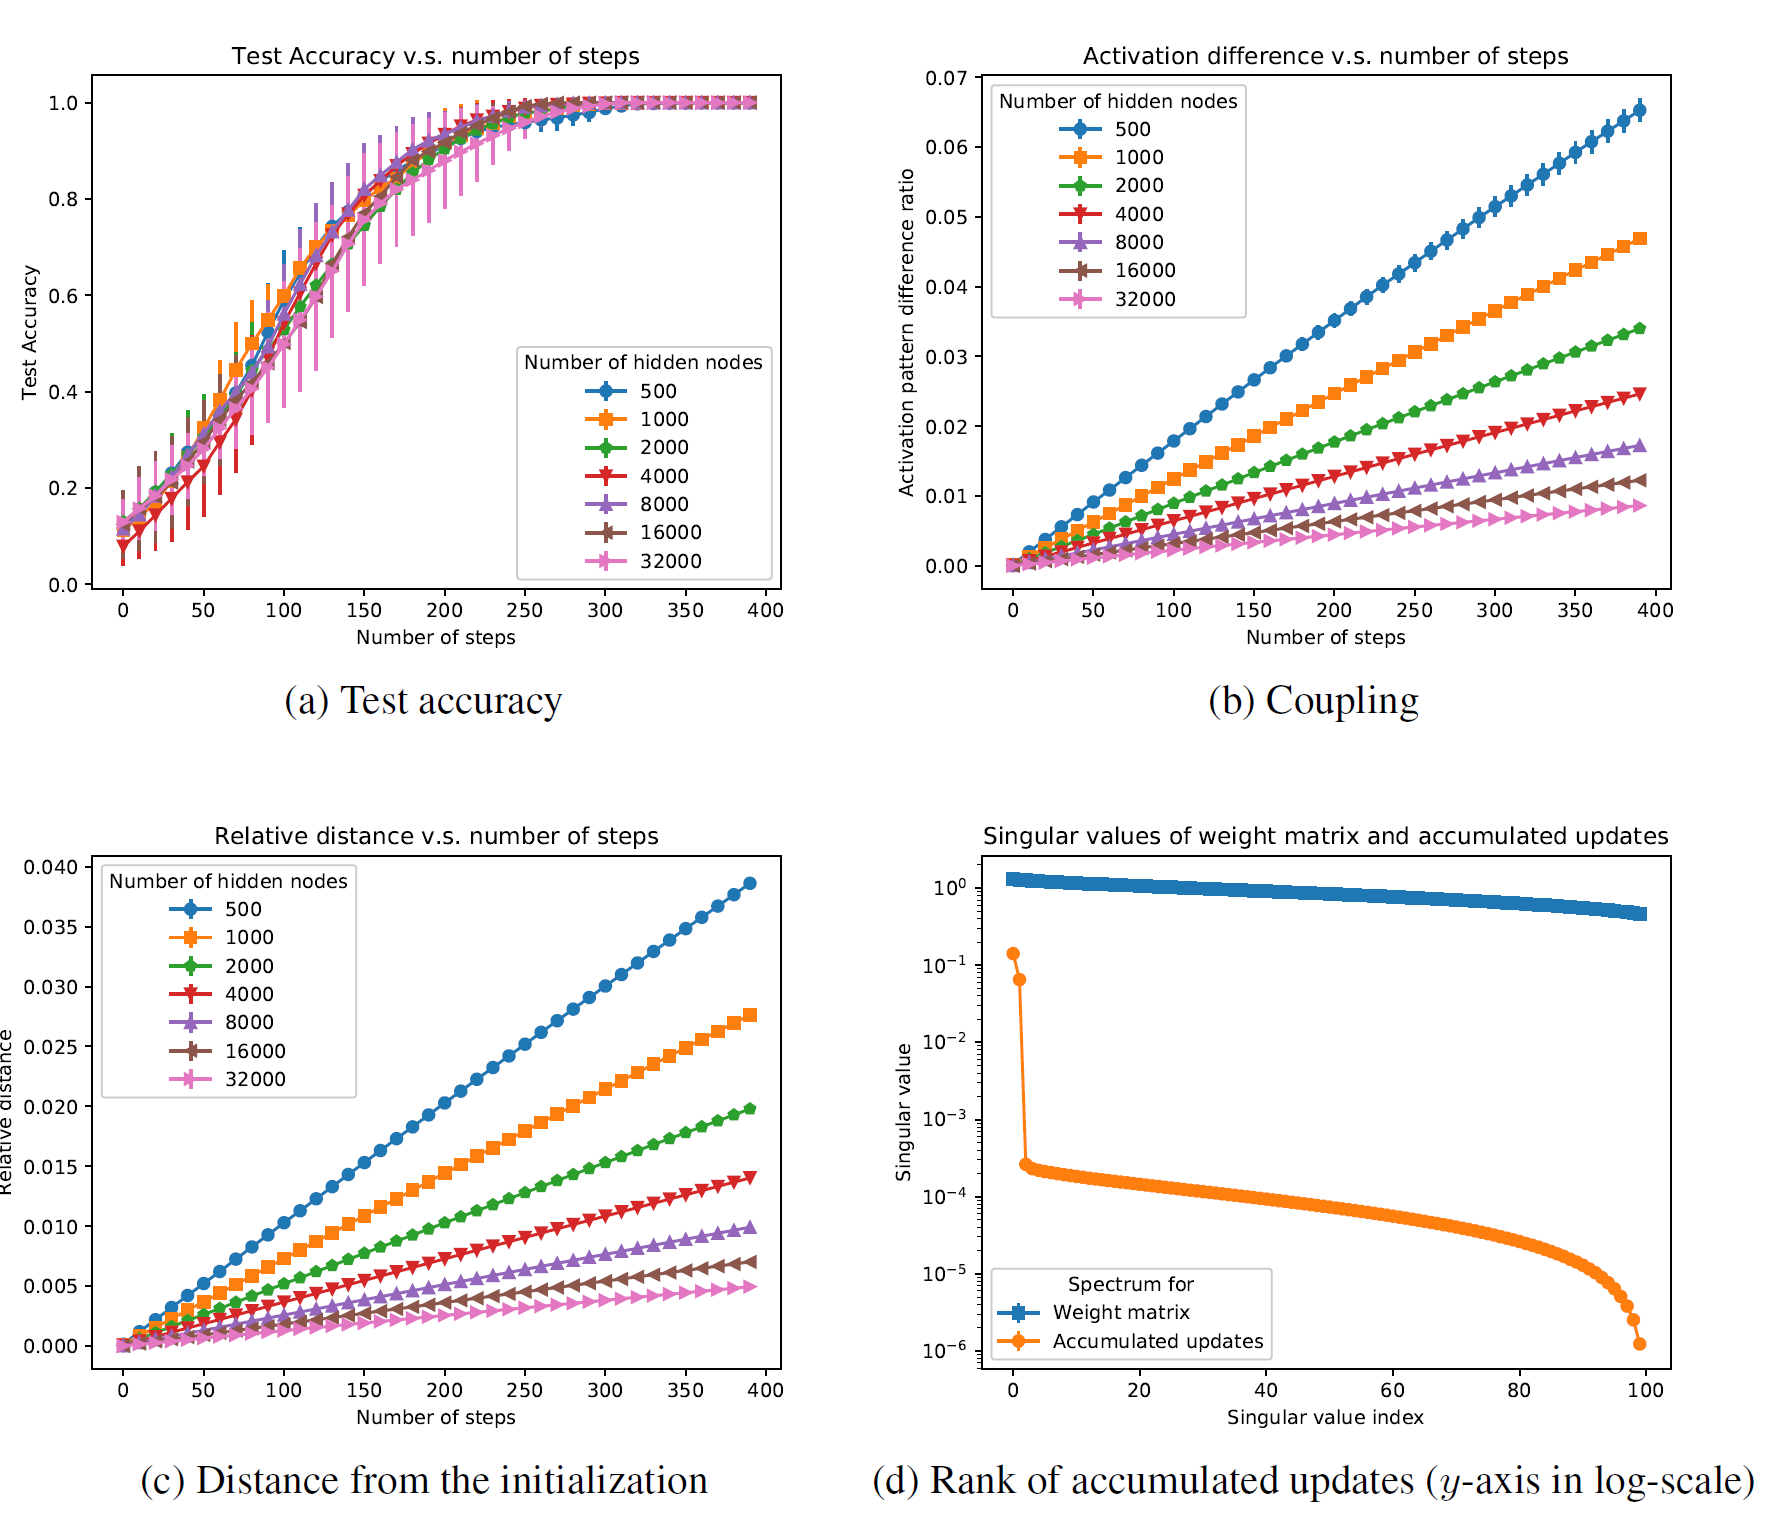
\includegraphics[width=12cm]{./figures/results.png}
\caption{在合成数据上的结果}
\end{figure}


\section{实验}
本节旨在验证一些关键含义:(1)隐藏单元的激活模式与初始化时的激活模式耦合;(2)与初始化的大小相比,从初始化到学习的解的距离相对较小;(3)累积的更新(即学习的权重矩阵之间的差异和初始化)具有近似低秩。合成数据和MNIST数据的结果确实支持这一点。附加实验见附录D。
\par
设置。合成数据是1000维的,由$k=10$个类组成,每个类都有$l=2$个分量。每个分量的概率均为$1/kl$,是协方差为$\sigma^2 / dI$的高斯分布,其平均值为从高斯分布$\mathcal{N}(0,\sigma^2_0 d)$中采样的i.i.d.,其中$\sigma = 1$和$\sigma_0 = 5$。抽取1000个训练数据点和1000个测试数据点。
\par
网络结构和学习过程遵循第3节;实验中隐藏单元$m$的个数变化,权值初始为$\mathcal{N}(0,1/m)$。在综合数据上,SGD运行为$T=400$步,批大小$B=16$,学习率$\eta = 10/m$。在MNIST上,SGD运行为$T=2×104$步,批大小$B=64$,学习率$\eta=4×103/m$。
\par
除了测试精度外,我们还报告了三个对应于待验证的三个观测/影响的量。首先,对于耦合,我们计算其激活模式与初始化时相比发生变化的隐藏单元的分数。这里,如果ReLU的输入为正,激活模式定义为1,否则定义为0。其次,对于距离,我们计算相对比率$\|w^{(t)} - w^{(0)}\|_F/\|w^{(0)}\|_F$,其中$w^{(t)}$是时间$t$时的权重矩阵。最后,对于累积更新的秩,我们绘制$w^{(T)}-w^{(0)}$的奇异值,其中$T$是最后一步。所有实验重复5次,并报告平均值和标准偏差。

\begin{figure}
\centering
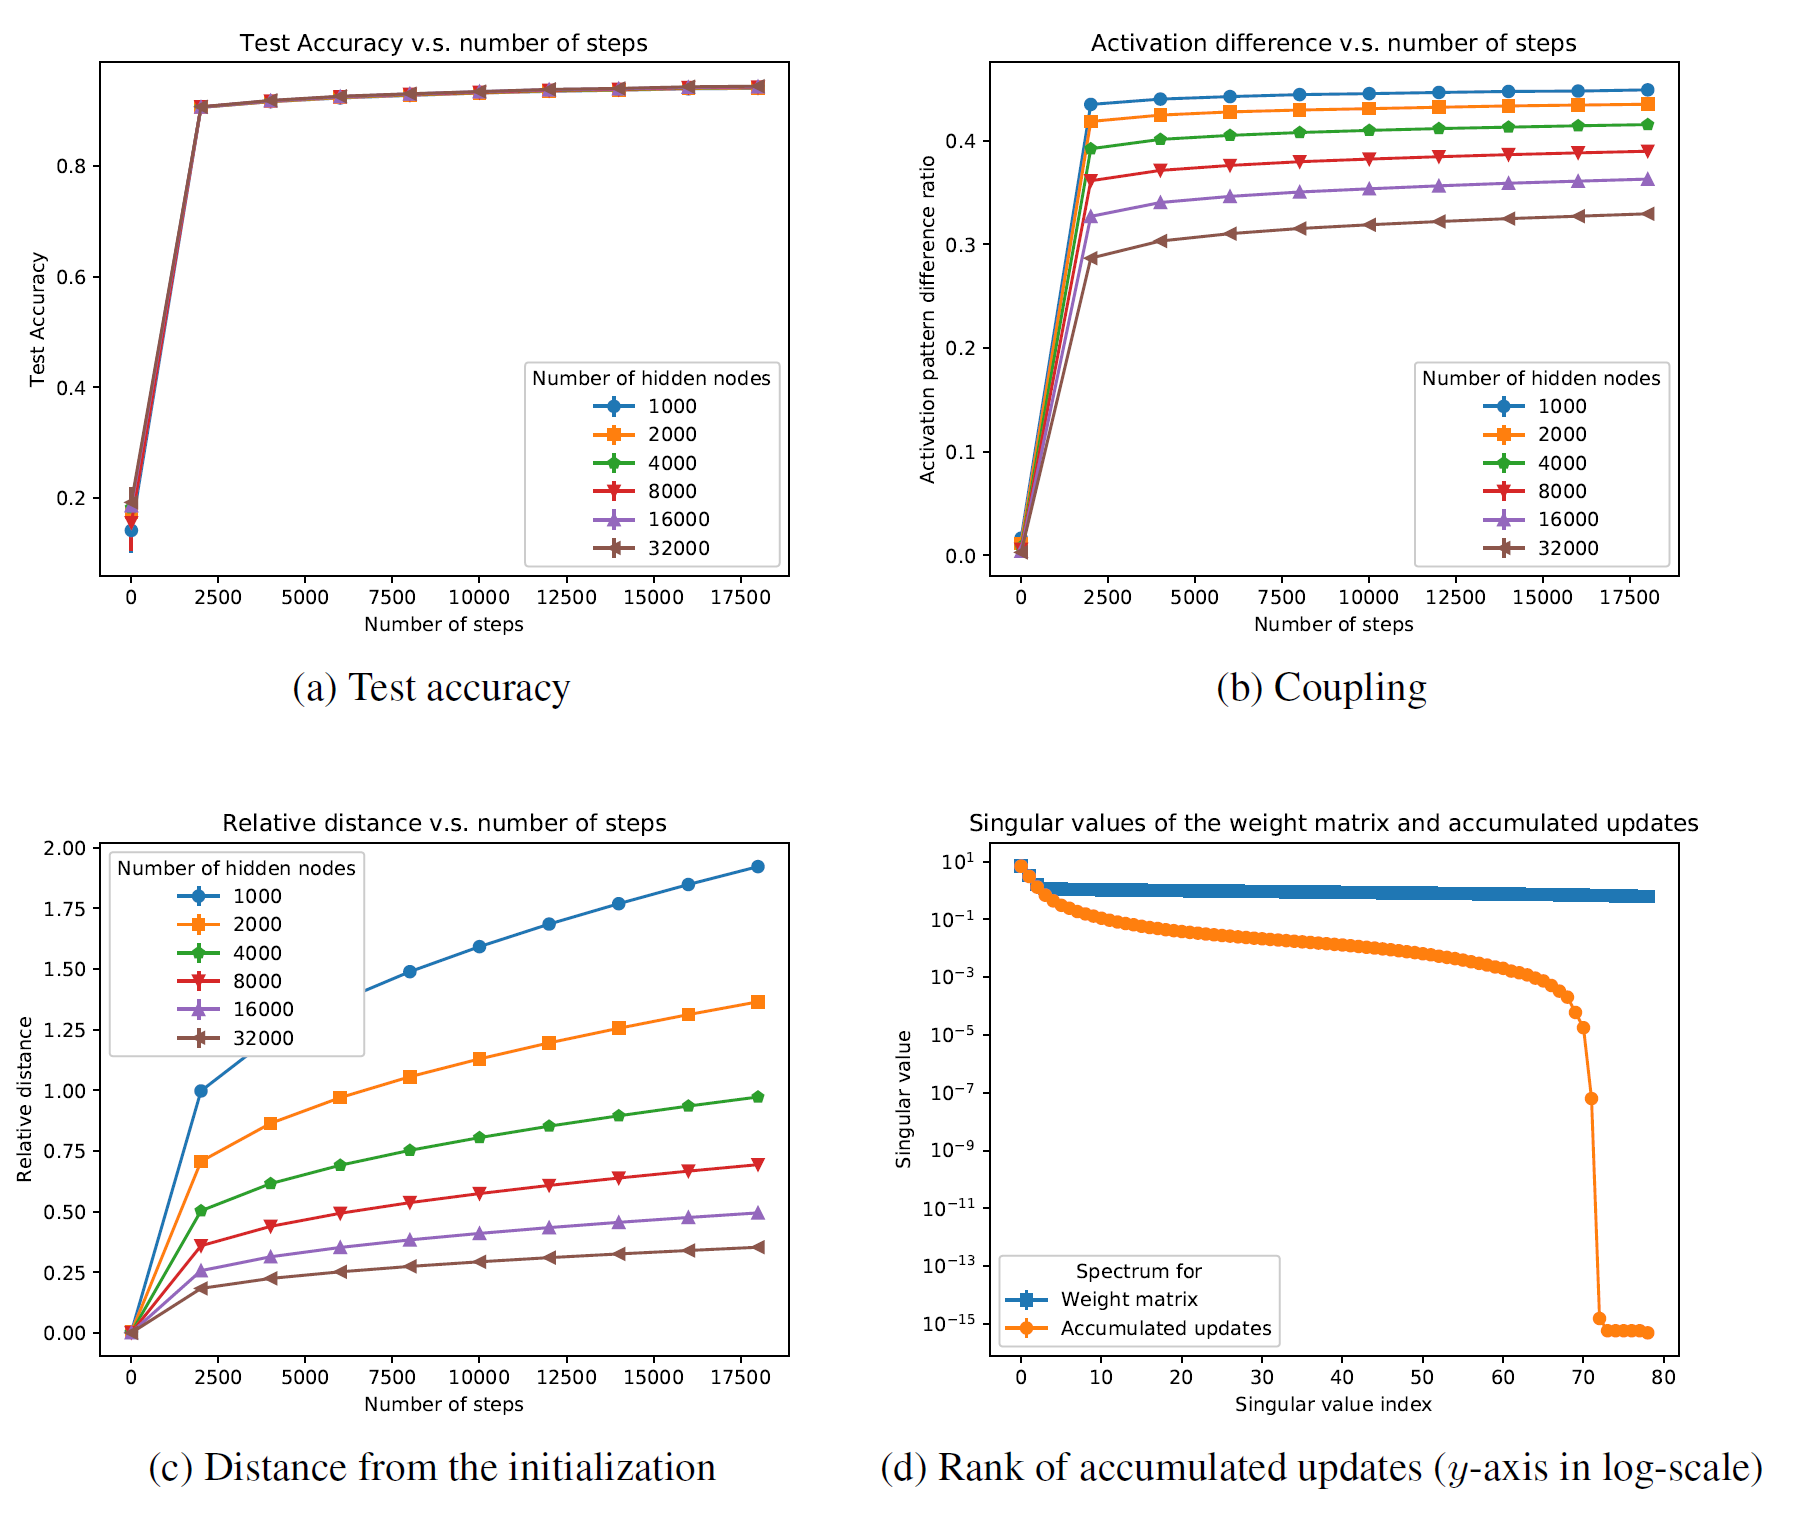
\includegraphics[width=12cm]{./figures/mnist.png}
\caption{在MNIST数据集上的结果}
\end{figure}
\par
结果。图1显示了合成数据的结果。测试精度很快收敛到100\%,隐单元数越大,测试精度越高,说明过参数化有助于优化和推广。回想一下,我们的分析表明,对于学习率随隐藏节点数$m$线性下降的情况,获得所需精度的迭代次数应该大致相同,这在这里也得到了验证。激活模式差比小于0.1,说明存在强耦合。相对距离小于0.1,因此最终的解决方案确实接近初始化。最后,累积更新的前20个奇异值比其余的大得多,而权重矩阵的谱没有这样的结构,这也与我们的分析一致。
\par
图2显示了MNIST上的结果。总体上,观察结果与合成数据上的观察结果相似(尽管不太显著),而且随着过度参数化,观察到的趋势也变得更加明显。附录中提供了一些额外的结果(例如,改变合成数据的方差),这些结果也支持我们的理论。

\section{结论}
本文研究了在实际数据集启发下,通过随机梯度下降(SGD)从随机初始化数据中学习两层超参数ReLU神经网络的问题。虽然我们的工作朝着神经网络训练的SGD的理论理解迈出了一步,但还远没有定论。特别是,对于不同于“2”的度量,甚至是某个流形给出的非凸距离,实际数据可以是可分离的。我们认为这是一个重要的开放方向。

\section{致谢}
我们要感谢NIPS'18的匿名评论员和Jason Lee的有益评论。这项工作部分得到了FA9550-18-1-0166、NSF拨款CCF-1527371、DMS-1317308、西蒙斯研究员奖、西蒙斯合作奖和ONR-N00014-16-1-2329的支持。梁颖宇也要感谢威斯康星大学麦迪逊分校研究和研究生教育副校长办公室在威斯康星校友研究基金会的资助下对这项研究的支持。